\subsection{x-project toolkit}

``Everything is an element'', from an AJAX request to an entire web page. Every part of the website is encapsulated inside an element. 

\brand{x-project} provide a set of Polymer element for local routing, API requests, User management, forms composition, layout and style. 

\subsubsection{Elements for local routing}
These elements can be used to perform local routing (for Single Page Application.

\vspace{0.2cm}

\texttt{<x-router>} implements local routing based on \emph{HTML5 Push State API}. 

\vspace{0.2cm}

\texttt{<x-route>} represents a route-to-page mapping. It has two input attributes: \texttt{route} and \texttt{page}. A route can be parametrized: parameters are sent as attributes to the corresponding page.

\vspace{0.2cm}

\texttt{<x-link>} is an extension of the anchor element \texttt{<a>} that prevents the default behavior when a click event occurs, blocking page request to the server and redirecting the request to the local router. 

\begin{lstlisting}[language=HTML5]
<link rel="import" 
  href="/elements/page-posts.html">
<link rel="import" 
  href="/elements/page-post.html">

<x-router>
  <x-route route="posts" page="posts">
  <x-route route="posts/:id" page="post">
</x-route>
\end{lstlisting}


\subsubsection{Elements for API requests}
These elements handle models API.

\texttt{<api-collection-get>} gets a collection of models. 

\begin{lstlisting}[language=HTML5]
<api-collection-get name="{{name}}" 
  filter="{{filter}}" 
  page="{{page}}" perpage="{{perpage}}"  
  collection="{{items}}" schema="{{schema}}"
  count="{{count}}">
</api-collection-get>
\end{lstlisting}

\texttt{<api-collection-post>} add a new model to the collection. 

\begin{lstlisting}[language=HTML5]
<api-collection-post name="{{name}}" 
  model="{{model}}"></api-collection-post>
\end{lstlisting}

\texttt{<api-collection-schema>} retrieve a model schema.

\begin{lstlisting}[language=HTML5]
<api-collection-schema name="{{name}}" 
  schema="{{schema}}"></api-collection-schema>
\end{lstlisting}

\texttt{<api-model-get>} retrieve a model. 
\texttt{<api-model-delete>} delete a model. 

\begin{lstlisting}[language=HTML5]
<api-model-get name="{{name}}" 
  model-id="{{model_id}}"
  model="{{model}}" schema="{{schema}}">
</api-model-get>
\end{lstlisting}

\texttt{<api-model-put>} retrieve a model. 

\begin{lstlisting}[language=HTML5]
<api-model-put name="{{name}}" 
  model="{{model}}"></api-model-put>
\end{lstlisting}


\subsubsection{Elements for lists and forms}
These elements are used to create forms (even dinamically from a schema). 

\texttt{<x-input>} is an extension of the input element. 
It's type can be \texttt{string}, \texttt{date}, \texttt{email}, \texttt{location},
\texttt{number}, \texttt{file}.

\begin{lstlisting}[language=HTML5]
<x-input type="{{type}}" label="{{label}}"
  value="{{value}}"></x-input>
\end{lstlisting}

\texttt{<x-form>} generate dinamically (from a model schema) a form to create/update a model.

\begin{lstlisting}[language=HTML5]
<x-form schema="schema" 
  model="{{model}}"></x-form>
\end{lstlisting}

\texttt{<x-filter>} generate dinamically (from a model schema) a form to create an API filter.

\begin{lstlisting}[language=HTML5]
<x-filter schema="{{schema}}"
  filter="{{filter}}"></api-filter>
\end{lstlisting}

\texttt{<x-table>} generate dinamically (froma a model schema) a table of models. 

\begin{lstlisting}[language=HTML5]
<x-table schema="{{schema}}" 
  collection="{{collection}}"></x-table>
\end{lstlisting}

\subsubsection{Elements for layout and style}

The style is based on \texttt{iron-flex-layout} \cite{iron-elements}, a CSS library of style mixins for cross-platform Flexible Box \cite{css-flexbox} layouts.




\subsubsection{Admin pages}

Client-side can be divided in two parts: \texttt{admin part} and \texttt{user part}.

The \emph{Admin part} is automatically generated. 
It consists of the following pages: \texttt{<page-collections>}, \texttt{<page-collection>} and \texttt{<page-model-edit>}.

\texttt{<page-collections>} is the admin main page. It shows the collections of the app. 

\begin{lstlisting}[language=HTML5]
<page-collections>
  <ul>
  <template items="{{collections}}">
    <li>
      <a is="x-link" href="/admin/{{item}}">
        {{item}}
      </a>
    </li>
  </template>
  </ul>
</page-collections>
\end{lstlisting}

\texttt{<page-collection>} shows the model instances of a collection.

\begin{lstlisting}[language=HTML5]
<page-collection>
  <api-collection-get name="{{collection}}" 
    filter="{{filter}}"
    collection="{{list}}">
  </api-collection-get>
  <x-filter schema="{{schema}}"
    filter="{{filter}}"></x-filter>
  <x-table schema="schema" 
    list="{{list}}">
  </x-table>
  <x-paginator current="{{page}}">
  </part-paginator>
</page-collection>
\end{lstlisting}

\texttt{<page-model-edit>} shows the forms to update a model.

\begin{lstlisting}[language=HTML5]
<page-model-edit>
  <api-model-get name="{{collection}}"
    model-id="model_id"
    model="{{model}}" schema="{{schema}}">
  </api-model-get>
  <x-form 
    schema="schema" model="model">
  </x-form>
  <api-model-put name="{{collection}}"
    model-id="{{model_id}}">
  </api-model-put>
</page-model-edit>
\end{lstlisting}

The \texttt{user part} depends on the type of the Web Application that has been implemented.
It is the part the final user interact with.

% \begin{figure}[!htbp]
% \centering
% 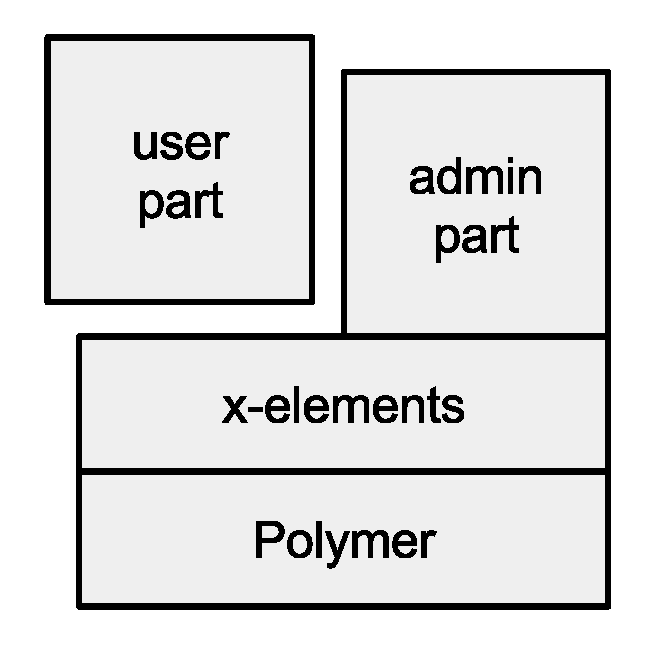
\epsfig{file=images/client-arch.eps, height=0.2\textwidth}
% \caption{Client-side architecture}
% \label{fig:client-arch}
% \end{figure}

